%%
%% This is file `example.tex',
%% generated with the docstrip utility.
%%
%% The original source files were:
%%
%% drexel-thesis.dtx  (with options: `example')
%% 
%% This is a generated file.
%% 
%% Copyright (C) 2010 W. Trevor King
%% 
%% This file may be distributed and/or modified under the conditions of
%% the LaTeX Project Public License, either version 1.3 of this license
%% or (at your option) any later version.  The latest version of this
%% license is in:
%% 
%%    http://www.latex-project.org/lppl.txt
%% 
%% and version 1.3 or later is part of all distributions of LaTeX version
%% 2003/06/01 or later.
%% 
%% See drexel-thesis.pdf for details.
\documentclass[subfig,blackref,approvalform]{drexel-thesis}

%% Enter the appropriate information here
\author{Hunter Kippen}
\title{New Methods for Detecting Frame Deletion in Modern Video}
\DUTmonth{May}
\DUTyear{2019}
\degree{Master of Science}
\advisor{Dr. Matthew Stamm, Ph.D.}
\copyrighttext{\copyrighttextCCBYSA}

\usepackage[super,sort&compress]{natbib} % fancy citation extensions
\bibliographystyle{unsrtnat}

\usepackage{fancyvrb} % nicer verbatim handling
\DefineShortVerb{\|}  % \verb+TEXT+  ->  |TEXT|

\renewenvironment{preamble}{% look, we're clobbering an environment!
  What preamble?\begingroup\color{white}}{\endgroup}

\usepackage[english]{babel} % English blindtext
\usepackage{blindtext} % macros for producing dummy output
\usepackage{amsmath}
\usepackage{amssymb}
\usepackage{dsfont}
\usepackage{bm}
\usepackage{subfig}

\DeclareMathOperator*{\argmin}{argmin}
\DeclareMathOperator*{\R}{\mathbb{R}}

\addto\captionsenglish{\DUTnames}

\begin{document}
\begin{DUTpreamble} % "DUT" because original preamble was clobbered.

\begin{dedications}

\Blindtext[3]
\end{dedications}

\begin{acknowledgments}
\Blindtext[3]
\end{acknowledgments}

\tableofcontents
\listoftables
\listoffigures

\begin{abstract}
\Blindtext[3]
\end{abstract}
\end{DUTpreamble}

\begin{thesis}
% This file is for the problem formulation section of the Master's Thesis.
% This file will not compile on it's own. Will need to include it into a main file
% That uses the drexel thesis template.
\chapter{Problem Formulation}

Detecting frame deletion in a video requires detecting the structural changes in a video due to the deletion process. In particular, Wang and Farid's work on temporal traces for detecting frame deletion shows that for MPEG-2 video, the P-frame prediction error can be formulated into a sequence. This sequence can then be monitored to detect frame deletion. Both Wang and Farid, and Stamm et al. use a system like in Fig.~\ref{System} to detect frame deletion. The prediction error sequence $e(n)$ is extracted from the decoded video file and processed to produce detection features. Wang and Farid's work did not propose features for automatic detection, and instead relied on visual inspection of the DFT of the prediction error sequence \cite{wang} \cite{stamm}.

\begin{figure}[htbp]
\centerline{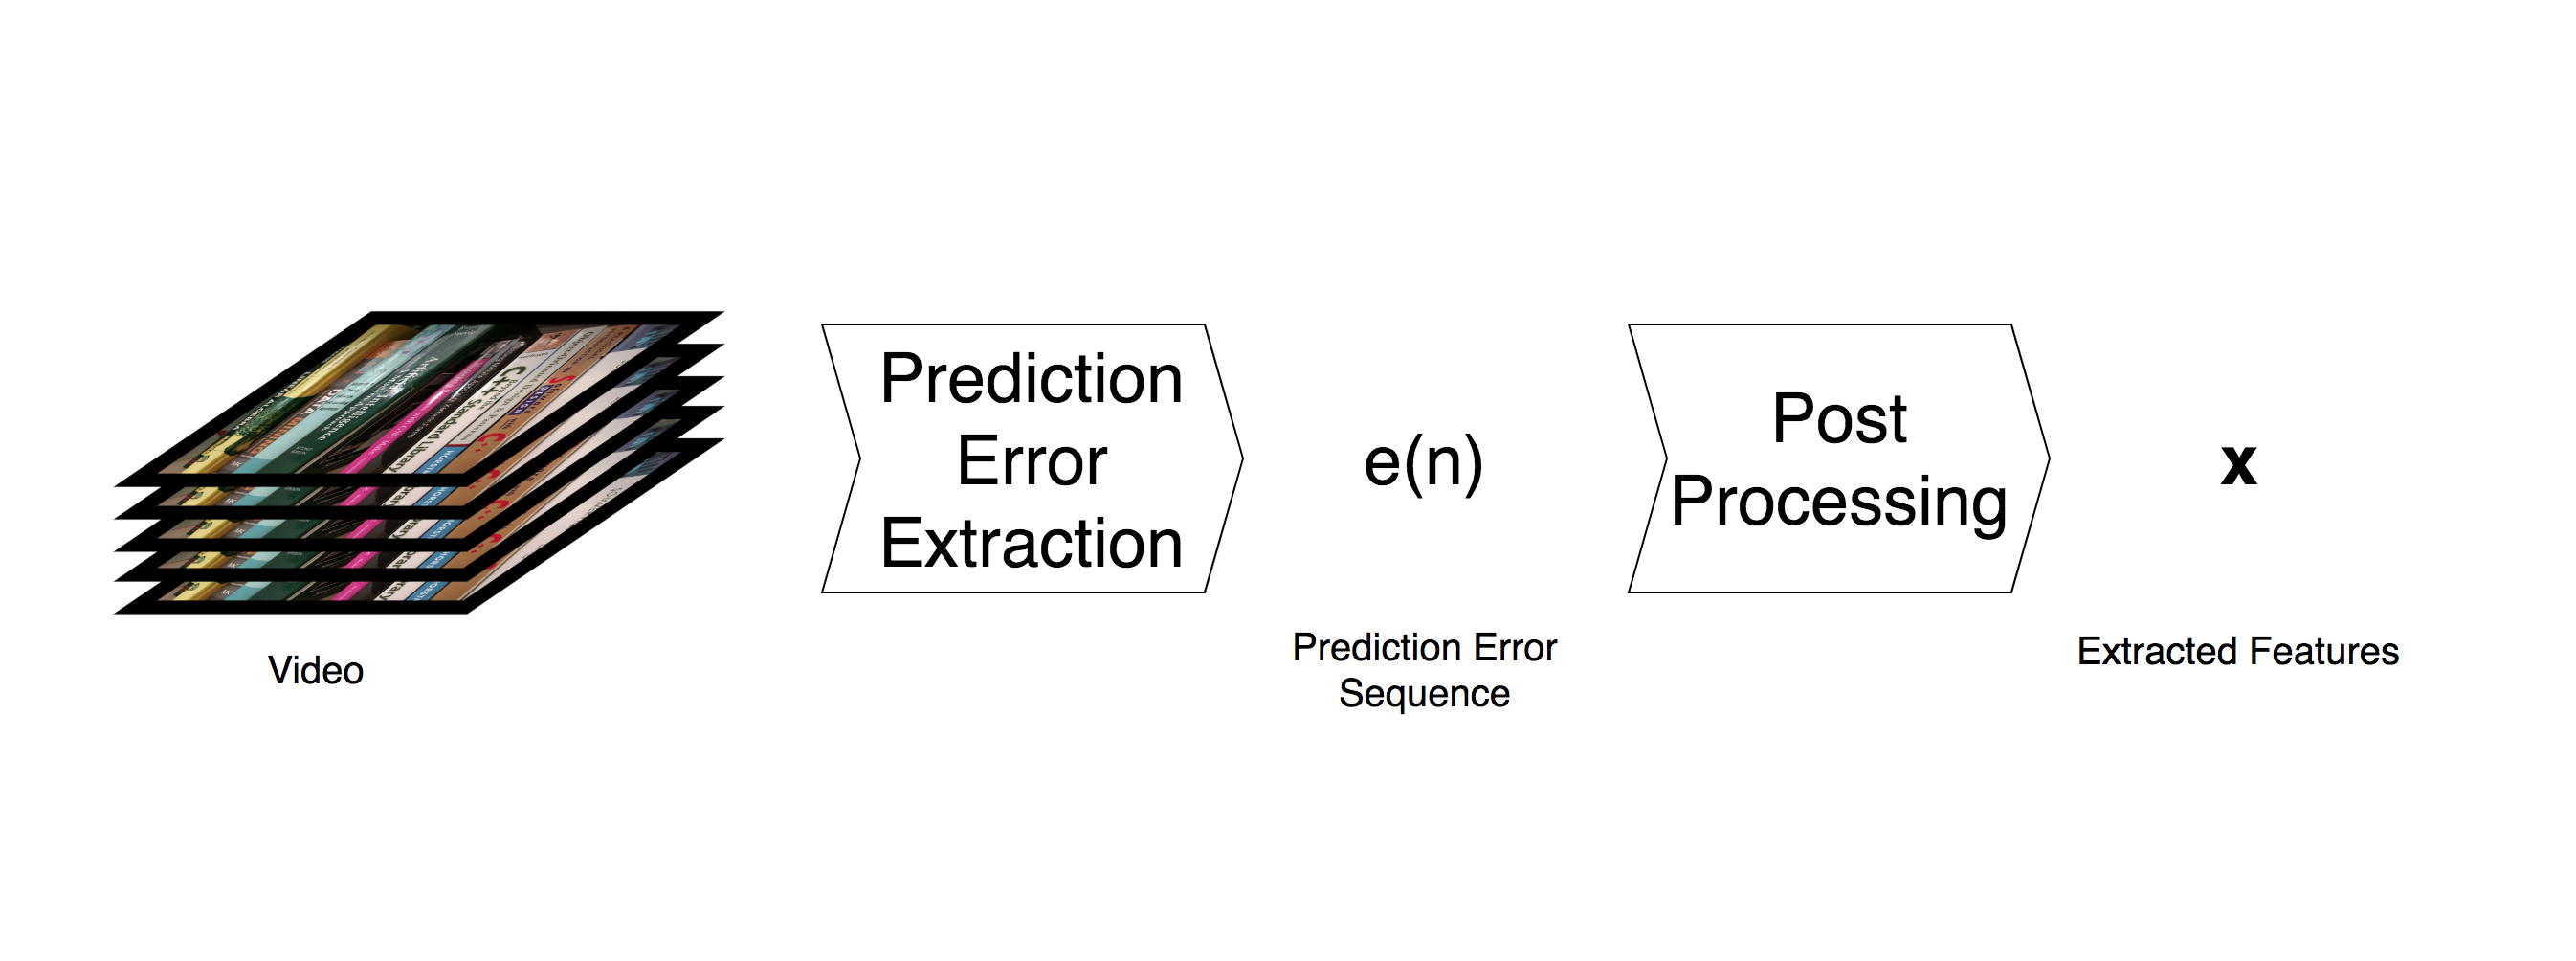
\includegraphics[width=0.9\linewidth]{ProblemFormulation/frame_deletion_detection_system.png}}
\caption{Generalized Approach to Frame Deletion Detection}
\label{System}
\end{figure}

This broad approach can also be applied to work with H.264 encoded video as well. While video encoding has advanced significantly, the fundamental structures of a compressed digital video have remained unchanged. Regardless of codec, the hallmark of video compression is the motion compensation and estimation process. Video frames are organized into GOPs that begin with an I-frame, and have varying structures of P and B-frames. In H.264, GOP structures are more dynamic due to the ability to derive motion-vector predictions from across multiple anchor frames. To remain robust to these advances in video compression, the prediction error extraction and post processing steps must be altered or augmented.

This work is concerned particularly with the detection of frame deletion in H.264 and similar modern video codecs. Frame addition has also been observed to introduce similar traces in the P-frame prediction error sequence as frame deletion. Our proposed system can be applied to detecting frame addition and for simplicity we will not discuss the detection of frame addition for the remainder of this thesis. We have made the following assumptions regarding our proposed system. First, we assume that all altered video has undergone re-compression. In fact, since most consumer video recording devices do not have the storage capability or processing power to record high-definition raw video, it is assumed that all video sources have been compressed by either MPEG-4 or H.264, and that all frame deleted video will be re-compressed using H.264 or a similar codec, where the reencoding is set to match the GOP structure of the source video. 

In addition, it is assumed that all videos that are passed to the detector are of sufficient length to make a classification. Without multiple full GOPs, the presence of a deletion fingerprint is negligible. Lastly, we make the assumption that if indeed frames have been removed from a video, they have not been removed from the end of the video. The detection features are dependent on differences between the structure of the prediction error sequences in natural videos versus videos with frame deletion. When frames are removed from the end of the video sequence, this difference is not observable. 

A user of our proposed system will not need physical access to a specific device to analyze a video captured by the device. The system should accept videos of an arbitrary length, and will not require metadata unrelated to video playback to be intact. It will work with videos of any resolution, frame rate, or GOP structure. Also, as our approach will be data driven, it is imperative that a user have access to a sufficient database of videos with known labels.

\section{Video Frame Deletion Detection}

Detecting frame deletion is a binary classification problem. Given a Video $V$, there are two possible classes:

\begin{equation}
\begin{aligned}
  C_{0} &: \text{The video is genuine, and has not had frames removed from it.} \\
  C_{1} &: \text{The video is altered, and has had frames removed from it.}
\end{aligned}
\end{equation}

Note that in this case, \emph{genuine} refers to the fact that the video has not undergone any additional post processing after its original capture. We will simply be considering the limited scenario whereby video has either come directly from the camera that captured it, or frames have been removed from the video and it has been recompressed. Any mention of a genuine video for the rest of this thesis refers to a video that has not been modified since it's original capture.

In general, it is difficult to classify whether or not a video has had frames removed based on the entirety of a video directly. Thus, the problem must be reworked. As shown above, a feature extraction system will be used to produce the P-frame prediction error sequence $e(n)$, and a feature vector $\bm{x}$. The feature vector ideally contains information about the prediction error sequence that can perfectly separate the two classes. As such, the classification problem is as follows. Given a feature vector $\bm{x}'$, it belongs to one of two classes:

\begin{equation}
\begin{aligned}
  C_{0} &: \bm{x}' \text{resulted from a genuine video that has not had frames removed from it.} \\
  C_{1} &: \bm{x}' \text{resulted from an altered video which has had frames removed from it.}
\end{aligned}
\end{equation}

In the following chapter, we will propose both a new method for extracting $e(n)$, and additional augmentations to $\bm{x}$ that allow for improved separation of data and increased robustness of the overall system.

\chapter{Proposed Approach}

\section{Prediction Error Sequence Extraction}

In previous work on frame deletion detection in MPEG-2, the prediction error sequence was extracted directly from the video decoder using the DCT coefficients of the prediction error residuals located in the compressed video file. The prediction error was averaged over all macroblocks in a frame. This prediction error was then stored as a sequence. Due to the nature of the correlation between P-frame prediction errors across a single GOP, any prediction made across GOP boundaries would result in increased prediction error. Wang and Farid showed that for fixed GOP video, the increase in average prediction error is periodic with respect to the number of frames deleted from the video. Stamm's work expands the idea of the prediction error trace by introducing the formulation of a fingerprint signal defined like so:

%TODO Put equations in for the definition of the the fingerprint signal s_hat

This fingerprint signal can be used to build a detector for both variable and fixed GOP videos. Despite this advance in detection, the underlying method for extracting the prediction error sequence is the same.

In MPEG-2, a P-frame is encoded by searching the previous anchor frame for the macroblock which incurs the least error. This means that the average prediction error for a single P-frame is only asssociated with the previous I or P-frame. H.264 expands the capabilities of its motion compensation and estimation system by allowing prediction from multiple previous frames (and subsequent frames in the case of B-frames). If the prediction error trace is extracted via the codec for H.264, the average prediction error associated with one frame is comprised of a linear combination of the average prediction error associated with motion vectors that map to the different anchor frames used in the motion estimation and compensation process. Thus, cross GOP predictions are smoothed out in such a way that it makes the fingerprint energy detector in Stamm's paper perform inadequately.

%TODO Put figure from stamm's paper showing the detection ROC
%TODO Show the detection ROC for the original methodology on H.264

As shown in Fig. ~\ref{•} the probability of detection using the methodology from MPEG-2 videos does not translate to H.264. Instead, we propose the following methodology for extracting the prediction error sequence in H.264.

\subsection{Proposed Prediction Error Sequence Extractor for H.264}

The goal of the proposed extraction algorithm is to maximize the probability that should frame deletion exist, a given measurement of the prediction error comes from a cross-GOP prediction. To this end, instead of directly measuring the prediction error from the DCT coefficients from the decoder, we decode the frame of interest and store the motion vectors associated with said frame. For each macroblock in the current frame, we use its associated motion vector to find the x and y coordinates defining the source macroblock which provides the least error mapping from a previous anchor frame. Then for a previous anchor frame, we subtract the pixels in the source macroblock from the destination macroblock in the current frame. This leaves us with a prediction error residual associated with the macroblock. We then calculate the average absolute value of this residual.

%TODO Insert Figure Showing Identification of Macroblocks in multiple previous frames

We repeat this process for each of D previous anchor frames. Then we store these prediction error values in a matrix $M$, where each row of the matrix corresponds to the errors associated with a single motion vector, and the columns are the errors associated with each of the previous anchor frames.

After obtaining the $M$ matrix for the current frame, we create the matrix $\tilde{M}$ defined like so:

\begin{equation}
  \tilde{M}_{i, j} = \mathds{1} \left(j == \argmin_{l} \left( M_{i, l} \right) \right) * M_{i, j}
\end{equation}

Thus $\tilde{M}$ is a copy of $M$ where the non-zero entries in each row correspond to the minimum average error associated with the macroblock and all other elements are zero. Effectively, the column index of the non-zero entry is an estimation of which previous frame the motion vector associated with the macroblock maps to in the decoding process.

Further processing is done on $\tilde{M}$ to output only a single prediction error value. First, $\tilde{M}$ is reduced into a vector $P$, such that:

\begin{equation}
  P_{j} = \frac{1}{N_{j}} \sum_{i}{\tilde{M}_{i,j}}
\end{equation}

Where $N_{j}$ is the number of non-zero elements in the $j^th$ column of $\tilde{M}$. Then, the reported prediction error $e$ is set as the maximum value of $P$. This entire process is repeated for every P frame in the video. This method of error extraction estimates which previous anchor frame contributes the maximum error per macroblock to the overall prediction error residual obtained by the codec for a given P frame. Since prediction across GOP boundaries results in spikes in the prediction error, the anchor frame that contributes the most error is most likely to be from a different original GOP. In this manner, we obtain a trace that is resilient to advances made in the motion compensation and estimation process in modern codecs as well as robust to variable frame rates and dynamic GOP structures.

\section{Proposed Detection Algorithm}

In addition to the new methods for prediction error extraction, we propose an expanded detection algorithm to better capture the statistical differences between videos. In fact, depending on scene content, video capture settings, and the amount of motion captured in a single recording, the prediction error sequence and fingerprint signal exhibit different structural behavior. This is true even for videos captured from a single camera model. Figure ~\ref{} shows this clearly. The two videos were captured from a *insert phone here* using the high quality 1080p capture mode. Both videos were shot using similar scene content, but the amount of motion in the video is different. The top row shows the different prediction error sequences, while the bottom row shows the fingerprint signals.

%TODO Insert figure comparing the two videos' fingerprint signals and prediction error seqs

Thus there is a need to construct a parametric model of the fingerprint signal and the prediction error sequence to capture these statistical variations. We propose constructing an autoregressive (AR) model of both the fingerprint signal and the prediction error sequence. Over the time period of one GOP it can be said that the signals are mostly stationary. The parameters of the AR models are added to a feature vector along with the fingerprint energy described above. In order to capture the degree to which this is true, the error variance of each AR model is also included. In addition, some basic statistical features are included to scale the overall decision surface. We propose including the mean and variance of both the prediction error sequence and fingerprint signal to the feature vector as well.

Note that after creating a feature vector for each video, the feature vector is quite large. It is inadvisable to create a probabilistic model of the feature vector for classification. Instead, we propose using a discriminative function to map an incoming feature vector directly to the set of natural videos or the set of videos altered by frame deletion. As such, we propose using a Support Vector Machine (SVM) classifier with a Radial Basis Kernel function for classification.
\end{thesis}

\bibliography{example-ref}

\appendix
%%
%% This is file `example-a.tex',
%% generated with the docstrip utility.
%%
%% The original source files were:
%%
%% drexel-thesis.dtx  (with options: `example-appendix')
%% 
%% This is a generated file.
%% 
%% Copyright (C) 2010 W. Trevor King
%% 
%% This file may be distributed and/or modified under the conditions of
%% the LaTeX Project Public License, either version 1.3 of this license
%% or (at your option) any later version.  The latest version of this
%% license is in:
%% 
%%    http://www.latex-project.org/lppl.txt
%% 
%% and version 1.3 or later is part of all distributions of LaTeX version
%% 2003/06/01 or later.
%% 
\chapter{Some Appendix Heading}
\Blindtext[5]
\chapter{Another Appendix Heading}
\Blindtext[5]
\endinput
%%
%% End of file `example-a.tex'.


\begin{vita}
\Blindtext[3]
\end{vita}

\end{document}
\endinput
%%
%% End of file `example.tex'.
